
\section{Comparison with the Hypothesis Corpus}
\label{sec:dataset-hc}

\begin{table}[t]
\centering
\begin{minipage}[t]{0.36\textwidth}
  \centering
  \caption{PBT corpus statistics.}
  \label{tab:dataset-stats}
  \footnotesize
  \begin{tabular}{lr}
    \toprule
    \textbf{Metric} & \textbf{Value} \\
    \midrule
    PBTs (raw scrape)              & 54{,}345 \\
    PBTs (post-dedup)              & 11{,}039 \\
    Unique repositories            & 333 \\
    Unique GitHub owners           & 281 \\
    Upstream project names         & 303 \\
    Top-1 / top-10 PBT share       & 8.7\% / 58.5\% \\
    \midrule
    \multicolumn{2}{@{}l}{\emph{Per-repo (min / med / max):}} \\
    PBTs per repo                  & 1 / 6 / 956 \\
    Stars                          & 0 / 0 / 9{,}438 \\
    Forks                          & 0 / 0 / 1{,}567 \\
    \midrule
    \multicolumn{2}{@{}l}{\emph{Per-PBT (min / med / max):}} \\
    PBT LoC                        & 2 / 13 / 174 \\
    Direct fn deps                 & 0 / 1 / 15 \\
    \bottomrule
  \end{tabular}
\end{minipage}\hfill
\begin{minipage}[t]{0.62\textwidth}
  \centering
  \setlength{\tabcolsep}{3pt}
  \caption{Comparison with HC-2026~\cite{devoe2026hypothesis}.}
  \label{tab:dataset-comparison}
  \footnotesize
  \begin{tabular}{@{}l c c@{}}
    \toprule
    & \textbf{\FVSpec:PBT} & \textbf{HC-2026} \\
    \midrule
    Discovery        & dep.\ graph        & GitHub search \\
    Raw PBTs         & 54{,}345           & 38{,}885 \\
    Tests (deduped)  & 11{,}039           & 23{,}139 \\
    Repos            & 333                & 1{,}504 \\
    Repo dedup       & fork/name          & \texttt{is\_fork} \\
    Test dedup       & SHA-256            & parametrization \\
    License filter   & no copyleft        & none \\
    Per-test data    & source + metrics   & runtime + coverage \\
    \midrule
    Repo overlap (valid)  & \multicolumn{2}{c}{28 / 333 \enskip(8\%)} \\
    Repo overlap (any)    & \multicolumn{2}{c}{111 / 333 \enskip(33\%)} \\
    \bottomrule
  \end{tabular}
\end{minipage}
\end{table}

While we were finalizing this work, the Hypothesis maintainers released their own scraped corpus~\cite{devoe2026hypothesis} (HC-2026).
The two corpora target different downstream uses---HC-2026 is built to study Hypothesis \emph{runtime} behavior (entropy consumption, predicate firing, coverage), while ours is built to feed a Lean formalization pipeline---which drives the design differences summarized in Table~\ref{tab:dataset-comparison}.
A consequence of HC-2026's runtime focus is that it filters out as ``invalid'' any repository whose PBTs may not be directly runnable without some custom setup: code that depends on external services, API keys, environment variables, or live databases. Our pipeline imposes no such requirement, since we only need a PBT's source code to translate it into Lean. Of our 333 repositories, 28 appear in HC-2026's valid (executable) set and 111 (33\%) appear in the pre-validity superset---meaning roughly 80 of our repositories were dropped by HC-2026 for being too operationally entangled to run, consistent with our goal of producing challenging and realistic FV problems.
Future work could merge the two corpora to enlarge the input pool; we did not pursue this here because the present token budget does not exhaust even our own 11{,}039-PBT corpus.

\section{\FVSpec:FV Grader Distributions}
\label{appndx:grader}

Figure~\ref{fig:difficulty_distribution} shows the difficulty distribution according to the Haiku 4.5 grader. Figure~\ref{fig:difficulty_vs_faithfulness} shows difficulty grade against output characteristics and lines of code.

\begin{figure}[t]
  \centering
  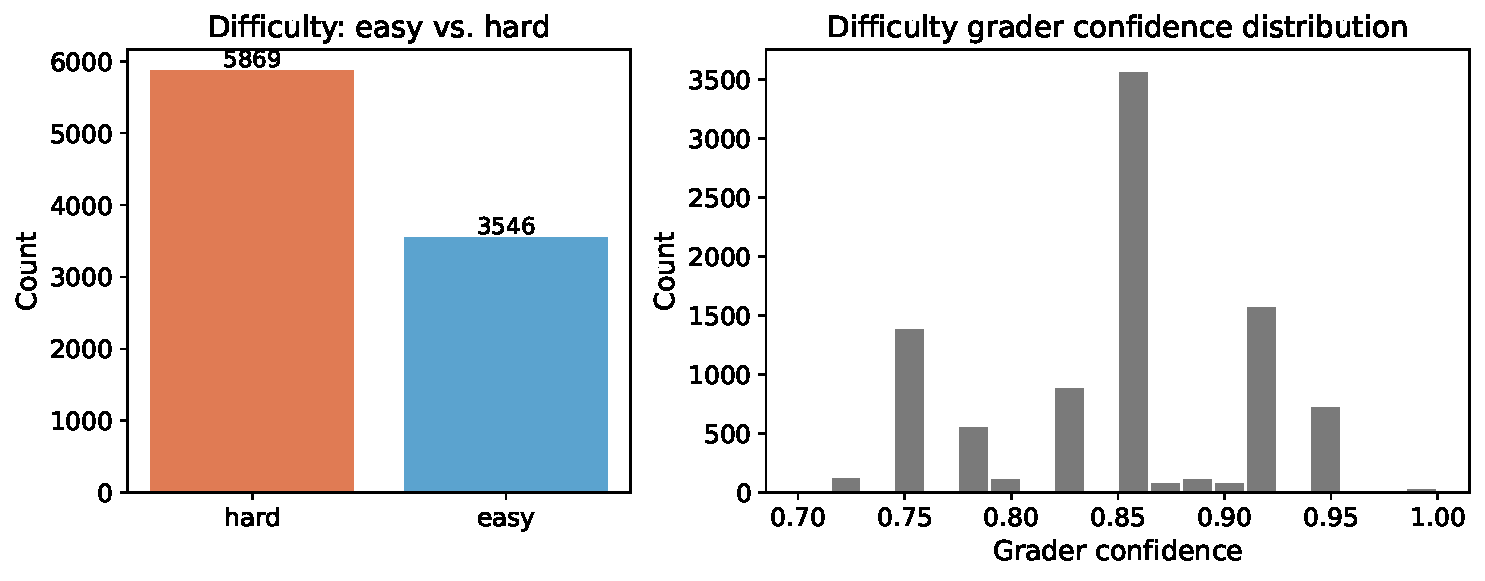
\includegraphics[width=\linewidth]{figs/difficulty_distribution.pdf}
  \caption{Difficulty distribution: easy vs.\ hard counts (left) and grader confidence distribution (right). $n$ shown in title.}
  \label{fig:difficulty_distribution}
\end{figure}

\begin{figure}[t]
  \centering
  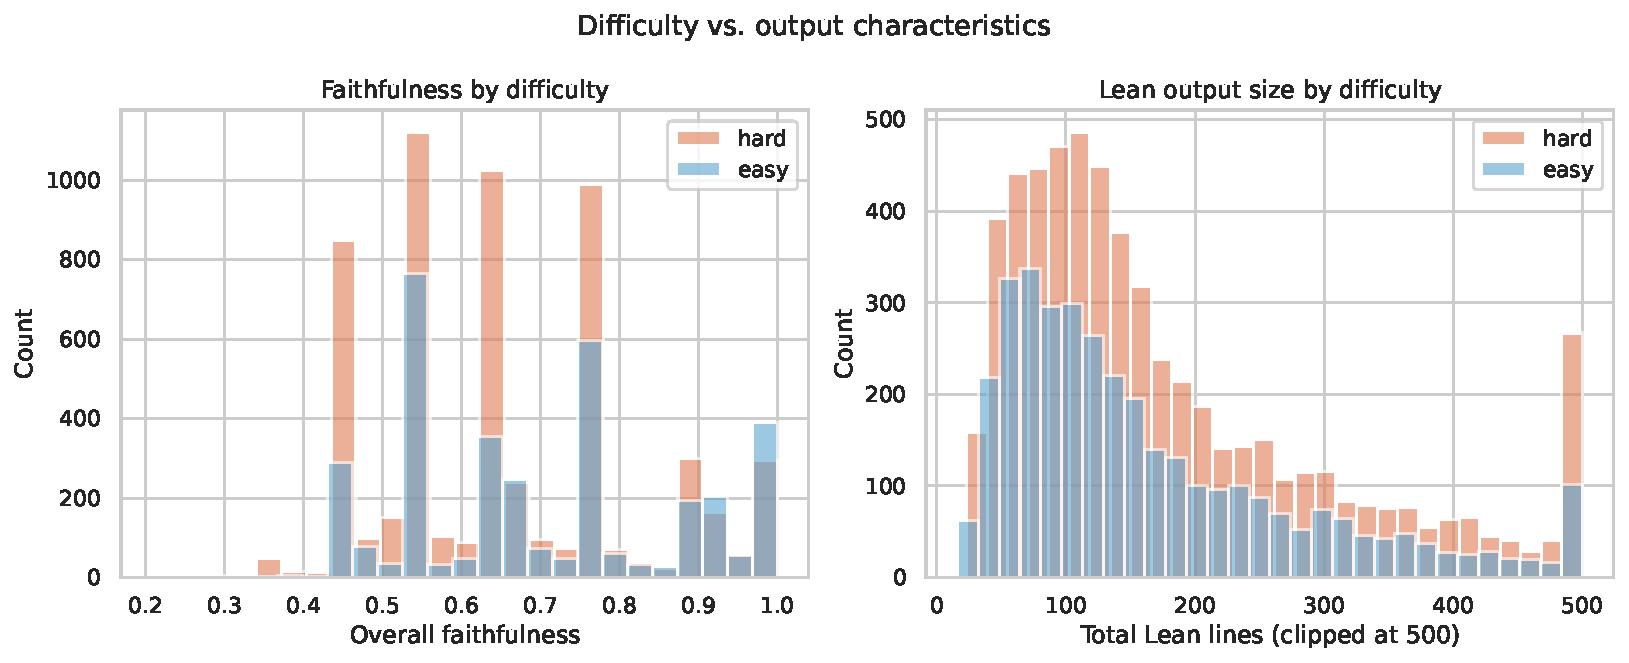
\includegraphics[width=\linewidth]{figs/difficulty_vs_faithfulness.pdf}
  \caption{Difficulty vs.\ output characteristics: overall faithfulness (left) and total Lean lines (right), stratified by difficulty.}
  \label{fig:difficulty_vs_faithfulness}
\end{figure}

\section{\FVSpec:FV Number of Theorems and Complexity per Sample}
\label{appndx:complexity}

Figure~\ref{fig:lean_complexity} shows the median sample contains multiple theorems each requiring an independent proof, and the \texttt{sorry} count tracks the theorem count closely, as expected from our pipeline design.

\begin{figure}[t]
  \centering
  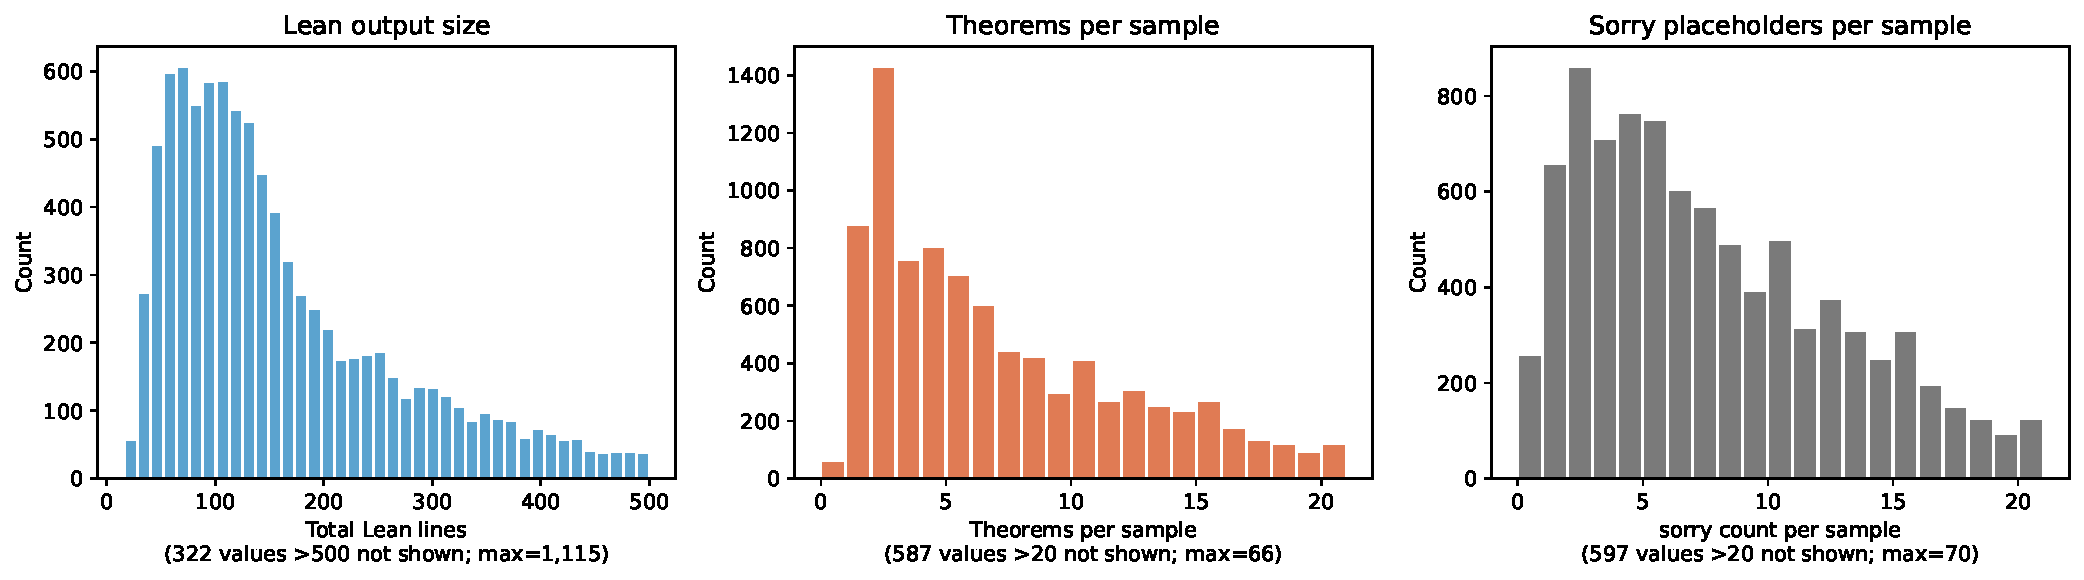
\includegraphics[width=\linewidth]{figs/lean_complexity.pdf}
  \caption{Lean output complexity: total lines (left), theorems per sample (center), and \texttt{sorry} placeholders per sample (right). Tail counts and maxima shown in axis labels.}
  \label{fig:lean_complexity}
\end{figure}

\section{\FVSpec:FV Pipeline Cost}
\label{appndx:pipeline_cost}

Per-sample pipeline cost is right-skewed (Figure~\ref{fig:pipeline_cost}): most samples compile within a few agent turns, but a tail of difficult translations requires many repair iterations before the Lean LSP reports success or the budget is exhausted.

\begin{figure}[t]
  \centering
  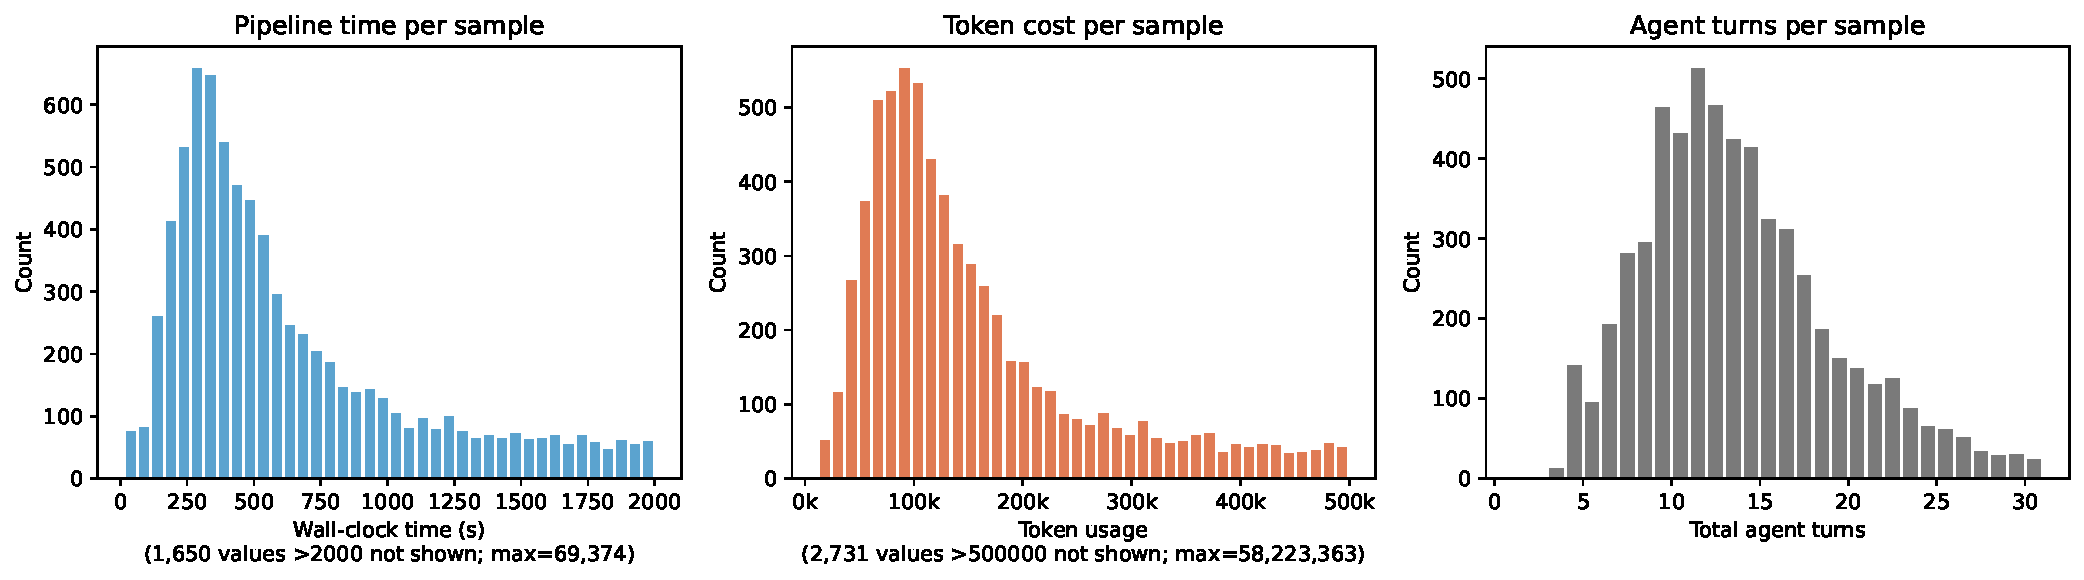
\includegraphics[width=\linewidth]{figs/pipeline_cost.pdf}
  \caption{Pipeline cost per sample: wall-clock time (left), token usage (center), and agent turns (right). Tail counts and maxima shown in axis labels.}
  \label{fig:pipeline_cost}
\end{figure}
